% Aufgabe 1 Binäre Suchbäume)
\begin{problemlist}

\pbitem{Induktion und binäre Bäume} \\
Ein binärer Baum heißt vollständig, falls jeder Knoten entweder null oder zwei Kinder besitzt.
\begin{enumerate}

\item Zeichnen Sie einen binären Suchbaum, der vollständig ist, und einen binären Suchbaum, der nicht vollständig ist.

\begin{answer}
\begin{itemize}
	\item Balancierter vollständiger BTS:
\end{itemize}
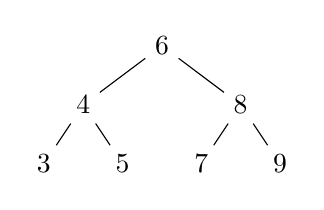
\begin{tikzpicture}[scale=0.5,
  level 1/.style={sibling distance=40mm},
  level 2/.style={sibling distance=20mm}]
\node{6}
	child{node{4}
		child{node{3}}
		child{node{5}}}
	child{node{8}
		child{node{7}}
		child{node{9}}};
\end{tikzpicture}

\begin{itemize}
	\item Unvollständiger BTS:
\end{itemize}

\begin{tikzpicture}[scale=0.5,
  level 1/.style={sibling distance=40mm},
  level 2/.style={sibling distance=20mm}]
\node{6}
	child{node{4}
		child{node{3}
			child{node{1}}
			child[missing]}
		child{node{5}}}
	child{node{8}
		child{node{7}}
		child{node{9}}};
\end{tikzpicture}

\end{answer}

\item Beweisen Sie durch eine geeignete Induktion: In jedem vollständigen binären Suchbaum ist die Anzahl der Blätter genau um eins größer als die Anzahl der inneren Knoten.

\begin{answer}
\begin{itemize}
	\item n jedem vollständigem BTS gilt: jeder Knoten n hat 0 oder genau 2 Kindknoten. 
    \item innerer Knoten: jeder Knoten v gilt als innerer Knoten gdw. v min. 1 Kindknoten hat.
    \item Blätter Knoten: Jeder Knoten v gilt als Blatt, wenn v keine Kinderknoten hat.
\end{itemize}

\textbf{Annahme:} In jedem vollständigen binären Suchbaum ist die Anzahl der Blätter genau um eins größer als die Anzahl der inneren Knoten. \\

base-case BTS mit einem inneren Knoten (root): \\
Angenommen der BTS erfüllt die Bedingungen eines vollständigen BTS und die Werte der Knoten spielen keine Rolle, dann muss gelten:  \\
$num_{\text{Blätter}}=num_{\text{innerer Knoten}}+1$


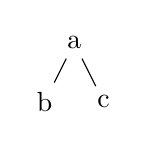
\begin{tikzpicture}[scale=0.5]
\node{a}
	child{node{b}}
	child{node{c}};
\end{tikzpicture}

Da die Werte in diesem Fall unerheblich sind, gilt die Zeichnung für einen vollständingen BTS mit einem inneren Knoten: \\
\begin{itemize}
	\item $num_{\text{innerer Knoten}}=a \text{ } num_{\text{innere Knoten}}=1$ 
	\item $num_{\text{Blätter}}=b,c \text{ } num_{\text{Blätter}}=2$ 
\end{itemize}

Die Anahme gilt im base-case. \\

\textbf{I.S:} Wenn die Annahme bei n inneren Knoten gilt, gilt sie auch $n+1$ inneren Knoten. 
Ein vollständiger BTS mit n inneren Knoten erfüllt die Gleichung:  \\
$num_{\text{Blätter}} = num_{\text{innerer Knoten}} + 1$ \\
Wenn es einen inneren Knoten zusätzlich geben soll, wird ein Blattknoten zu diesem Knoten und bekommt nach der Definition von vollständigen BTS 2 neue Kindknoten, da:

\begin{enumerate}
	\item nur 1 Kind Widerspruch mit Definition von vollständigen BTS.
	\item 0 Kindknoten, dann bleibt $num_{\text{innerer Knoten}}$ gleich, da das Blatt nicht zum Inneren Knoten werden konnte.
\end{enumerate}

\end{answer}


\item Formulieren Sie eine ähnliche Aussage für allgemeine binäre Suchbäume und beweisen Sie sie.

\textbf{Annahme/Eigenschaft:} In einem Baum gilt:$num_{node} = num_{edges} + 1$ $\Rightarrow$ die Anzahl der Knoten i m Baum ergibt sich aus Anzahl der Kanten + 1.
\begin{itemize}
	\item Jeder Knoten ist durch genau eine Kante mit seinem Elternknoten verbunden.
	\item Bei Insertion wird ein neuer Knoten mit seinem Elternknoten verbunden.
\end{itemize}

base-case: $num_{nodes} = 3$

\begin{tikzpicture}[scale=0.5]
\node{a}
	child[missing]
	child{node{b}
		child[missing]		
		child{node{c}}};
\end{tikzpicture}

$num_{Knoten} = \{a,b,c,\}$ $|num_{Knoten}| = 3$ \\
$num_{Kanten} = \{a-b,b-c\}$ $|num_{Kanten}| = 2$ \\
es gilt: $num_{node} = num_{edges} + 1$ $\Rightarrow$ $3 = 2 + 1$ \\
Die Annahme gilt für den base-case. \\

\textbf{I.S:} Wenn die Annahme bei n inneren Knoten gilt, gilt sie auch n+1 inneren Knoten. 
Ein Baum mit n inneren Knoten erfüllt die Gleichung: $num_{Knoten} = num_{Kanten} + 1$ \\ . Bei $n+1$ Knoten muss ein zusätzlicher Knoten in den Baum eingefügt werden (insertion). Durch den neuen Knoten einstehet immer eine neue Kanten, da ein Knoten nur EIN linkes und rechtes haben kann. ein Knoten kann nicht zwei linke oder rechte Knoten haben. Daher gilt: \\
\begin{enumerate}
	\item Hat der neue Knoten denselben Wert, wie ein anderer Knoten, so wird der alte durch den neuen ersetzt. $\Rightarrow$ immer noch n Knoten Gleichung bleibt unverändert und gilt daher immer noch.
	\item Der neue Knoten wird zum Kind eines anderen Knotens und mit einer neuen Kanten mit diesem Elternknoten verbunden. $\Rightarrow$ $n = n+1$  für die Gleichung gilt: $num_{Knoten} + 1 = num_{Kanten} + 1 + 1 = num_{Knoten} + 1 = num_{Kanten} + 2 \equiv num_{Knoten} = num_{Kanten} + 1$
	\item Die Annahme gilt für $n+1$
\end{enumerate}
\begin{flushright}
$\Box$
\end{flushright}


\end{enumerate}
